% Options for packages loaded elsewhere
\PassOptionsToPackage{unicode}{hyperref}
\PassOptionsToPackage{hyphens}{url}
%
\documentclass[
]{report}
\usepackage{amsmath,amssymb}
\usepackage{lmodern}
\usepackage{iftex}
\ifPDFTeX
  \usepackage[T1]{fontenc}
  \usepackage[utf8]{inputenc}
  \usepackage{textcomp} % provide euro and other symbols
\else % if luatex or xetex
  \usepackage{unicode-math}
  \defaultfontfeatures{Scale=MatchLowercase}
  \defaultfontfeatures[\rmfamily]{Ligatures=TeX,Scale=1}
\fi
% Use upquote if available, for straight quotes in verbatim environments
\IfFileExists{upquote.sty}{\usepackage{upquote}}{}
\IfFileExists{microtype.sty}{% use microtype if available
  \usepackage[]{microtype}
  \UseMicrotypeSet[protrusion]{basicmath} % disable protrusion for tt fonts
}{}
\makeatletter
\@ifundefined{KOMAClassName}{% if non-KOMA class
  \IfFileExists{parskip.sty}{%
    \usepackage{parskip}
  }{% else
    \setlength{\parindent}{0pt}
    \setlength{\parskip}{6pt plus 2pt minus 1pt}}
}{% if KOMA class
  \KOMAoptions{parskip=half}}
\makeatother
\usepackage{xcolor}
\usepackage{color}
\usepackage{fancyvrb}
\newcommand{\VerbBar}{|}
\newcommand{\VERB}{\Verb[commandchars=\\\{\}]}
\DefineVerbatimEnvironment{Highlighting}{Verbatim}{commandchars=\\\{\}}
% Add ',fontsize=\small' for more characters per line
\usepackage{framed}
\definecolor{shadecolor}{RGB}{248,248,248}
\newenvironment{Shaded}{\begin{snugshade}}{\end{snugshade}}
\newcommand{\AlertTok}[1]{\textcolor[rgb]{0.94,0.16,0.16}{#1}}
\newcommand{\AnnotationTok}[1]{\textcolor[rgb]{0.56,0.35,0.01}{\textbf{\textit{#1}}}}
\newcommand{\AttributeTok}[1]{\textcolor[rgb]{0.77,0.63,0.00}{#1}}
\newcommand{\BaseNTok}[1]{\textcolor[rgb]{0.00,0.00,0.81}{#1}}
\newcommand{\BuiltInTok}[1]{#1}
\newcommand{\CharTok}[1]{\textcolor[rgb]{0.31,0.60,0.02}{#1}}
\newcommand{\CommentTok}[1]{\textcolor[rgb]{0.56,0.35,0.01}{\textit{#1}}}
\newcommand{\CommentVarTok}[1]{\textcolor[rgb]{0.56,0.35,0.01}{\textbf{\textit{#1}}}}
\newcommand{\ConstantTok}[1]{\textcolor[rgb]{0.00,0.00,0.00}{#1}}
\newcommand{\ControlFlowTok}[1]{\textcolor[rgb]{0.13,0.29,0.53}{\textbf{#1}}}
\newcommand{\DataTypeTok}[1]{\textcolor[rgb]{0.13,0.29,0.53}{#1}}
\newcommand{\DecValTok}[1]{\textcolor[rgb]{0.00,0.00,0.81}{#1}}
\newcommand{\DocumentationTok}[1]{\textcolor[rgb]{0.56,0.35,0.01}{\textbf{\textit{#1}}}}
\newcommand{\ErrorTok}[1]{\textcolor[rgb]{0.64,0.00,0.00}{\textbf{#1}}}
\newcommand{\ExtensionTok}[1]{#1}
\newcommand{\FloatTok}[1]{\textcolor[rgb]{0.00,0.00,0.81}{#1}}
\newcommand{\FunctionTok}[1]{\textcolor[rgb]{0.00,0.00,0.00}{#1}}
\newcommand{\ImportTok}[1]{#1}
\newcommand{\InformationTok}[1]{\textcolor[rgb]{0.56,0.35,0.01}{\textbf{\textit{#1}}}}
\newcommand{\KeywordTok}[1]{\textcolor[rgb]{0.13,0.29,0.53}{\textbf{#1}}}
\newcommand{\NormalTok}[1]{#1}
\newcommand{\OperatorTok}[1]{\textcolor[rgb]{0.81,0.36,0.00}{\textbf{#1}}}
\newcommand{\OtherTok}[1]{\textcolor[rgb]{0.56,0.35,0.01}{#1}}
\newcommand{\PreprocessorTok}[1]{\textcolor[rgb]{0.56,0.35,0.01}{\textit{#1}}}
\newcommand{\RegionMarkerTok}[1]{#1}
\newcommand{\SpecialCharTok}[1]{\textcolor[rgb]{0.00,0.00,0.00}{#1}}
\newcommand{\SpecialStringTok}[1]{\textcolor[rgb]{0.31,0.60,0.02}{#1}}
\newcommand{\StringTok}[1]{\textcolor[rgb]{0.31,0.60,0.02}{#1}}
\newcommand{\VariableTok}[1]{\textcolor[rgb]{0.00,0.00,0.00}{#1}}
\newcommand{\VerbatimStringTok}[1]{\textcolor[rgb]{0.31,0.60,0.02}{#1}}
\newcommand{\WarningTok}[1]{\textcolor[rgb]{0.56,0.35,0.01}{\textbf{\textit{#1}}}}
\usepackage{longtable,booktabs,array}
\usepackage{calc} % for calculating minipage widths
% Correct order of tables after \paragraph or \subparagraph
\usepackage{etoolbox}
\makeatletter
\patchcmd\longtable{\par}{\if@noskipsec\mbox{}\fi\par}{}{}
\makeatother
% Allow footnotes in longtable head/foot
\IfFileExists{footnotehyper.sty}{\usepackage{footnotehyper}}{\usepackage{footnote}}
\makesavenoteenv{longtable}
\usepackage{graphicx}
\makeatletter
\def\maxwidth{\ifdim\Gin@nat@width>\linewidth\linewidth\else\Gin@nat@width\fi}
\def\maxheight{\ifdim\Gin@nat@height>\textheight\textheight\else\Gin@nat@height\fi}
\makeatother
% Scale images if necessary, so that they will not overflow the page
% margins by default, and it is still possible to overwrite the defaults
% using explicit options in \includegraphics[width, height, ...]{}
\setkeys{Gin}{width=\maxwidth,height=\maxheight,keepaspectratio}
% Set default figure placement to htbp
\makeatletter
\def\fps@figure{htbp}
\makeatother
\setlength{\emergencystretch}{3em} % prevent overfull lines
\providecommand{\tightlist}{%
  \setlength{\itemsep}{0pt}\setlength{\parskip}{0pt}}
\setcounter{secnumdepth}{5}
\newlength{\cslhangindent}
\setlength{\cslhangindent}{1.5em}
\newlength{\csllabelwidth}
\setlength{\csllabelwidth}{3em}
\newlength{\cslentryspacingunit} % times entry-spacing
\setlength{\cslentryspacingunit}{\parskip}
\newenvironment{CSLReferences}[2] % #1 hanging-ident, #2 entry spacing
 {% don't indent paragraphs
  \setlength{\parindent}{0pt}
  % turn on hanging indent if param 1 is 1
  \ifodd #1
  \let\oldpar\par
  \def\par{\hangindent=\cslhangindent\oldpar}
  \fi
  % set entry spacing
  \setlength{\parskip}{#2\cslentryspacingunit}
 }%
 {}
\usepackage{calc}
\newcommand{\CSLBlock}[1]{#1\hfill\break}
\newcommand{\CSLLeftMargin}[1]{\parbox[t]{\csllabelwidth}{#1}}
\newcommand{\CSLRightInline}[1]{\parbox[t]{\linewidth - \csllabelwidth}{#1}\break}
\newcommand{\CSLIndent}[1]{\hspace{\cslhangindent}#1}
\usepackage{booktabs}
\usepackage{geometry}
\usepackage[none]{hyphenat}
\usepackage{titlesec}
\usepackage{longtable}
\usepackage{xcolor}
\usepackage{setspace}
\usepackage{pdfpages}

\pagestyle{plain}

%%%% Set margins
\setlength{\topmargin}{-1cm}
\addtolength{\evensidemargin}{-1cm}
\addtolength{\oddsidemargin}{-1cm}
\addtolength{\textheight}{3cm}
\addtolength{\textwidth}{2cm}

% Spacing for reading guides
\newcommand{\rgs}{\vspace{12pt}} % Vertical space
\newcommand{\rgi}{\hspace{24pt}}  % Indent

\newcommand\latexcode[1]{#1}

% Format chapter titles and spacing
\renewcommand*{\chaptername}{Week}

\titleformat{\chapter}[display]
{\bfseries\Large}
{\filleft\MakeUppercase{\chaptertitlename} \Huge\thechapter}
{3ex}
{\titlerule
\vspace{1.5ex}%
\filright}
[\vspace{1.5ex}%
\titlerule]
\titlespacing*{\chapter}{0pt}{-40pt}{20pt}
\ifLuaTeX
  \usepackage{selnolig}  % disable illegal ligatures
\fi
\IfFileExists{bookmark.sty}{\usepackage{bookmark}}{\usepackage{hyperref}}
\IfFileExists{xurl.sty}{\usepackage{xurl}}{} % add URL line breaks if available
\urlstyle{same} % disable monospaced font for URLs
\hypersetup{
  hidelinks,
  pdfcreator={LaTeX via pandoc}}

\title{\textbf{STAT 216 Coursepack}\\
\strut \\
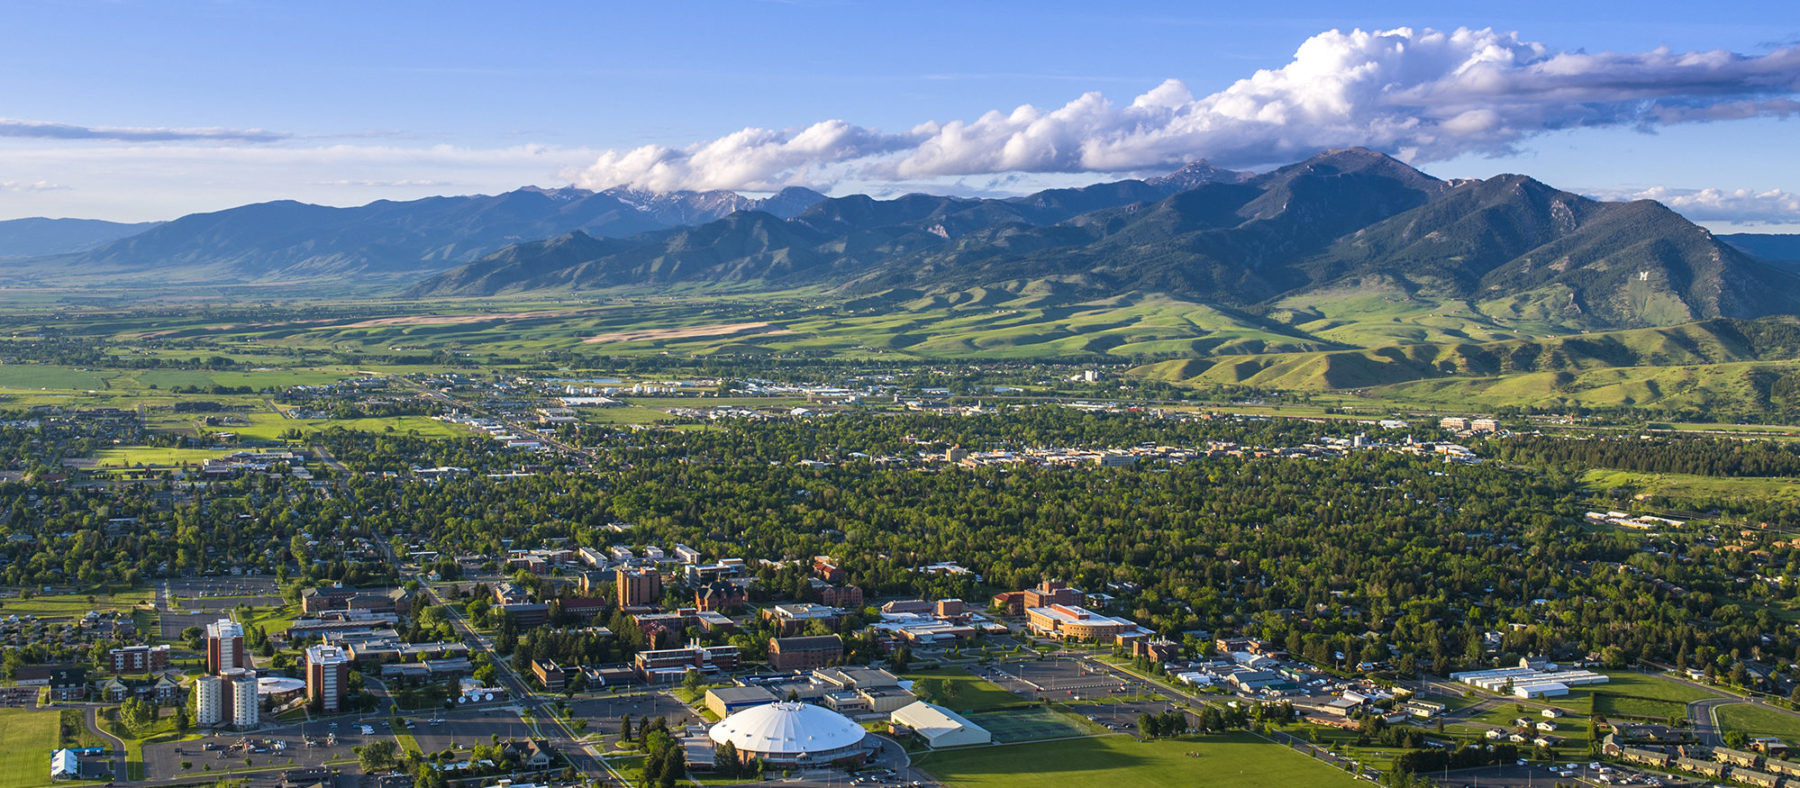
\includegraphics[width=5in,height=\textheight]{images/msu-campus.jpg}}
\usepackage{etoolbox}
\makeatletter
\providecommand{\subtitle}[1]{% add subtitle to \maketitle
  \apptocmd{\@title}{\par {\large #1 \par}}{}{}
}
\makeatother
\subtitle{Fall 2022\\
Montana State University}
\author{Melinda Yager\\
Jade Schmidt\\
Stacey Hancock}
\date{}

\begin{document}
\maketitle

\newpage
\thispagestyle{empty}

This resource was developed by Melinda Yager, Jade Schmidt, and Stacey Hancock in 2021 to accompany the online textbook: Carnegie, N., Hancock, S., Meyer, E., Schmidt, J., and Yager, M. (2021). \emph{Montana State Introductory Statistics with R}. Montana State University. \url{https://mtstateintrostats.github.io/IntroStatTextbook/}.

This resource is released under a \href{https://creativecommons.org/licenses/by-nc-sa/4.0/}{Creative Commons BY-NC-SA 4.0} license unless otherwise noted.

\setcounter{tocdepth}{1}
\addtocontents{toc}{\protect\thispagestyle{empty}}
\tableofcontents
\thispagestyle{empty}

\newpage
\setcounter{page}{1}

\hypertarget{preface}{%
\chapter*{Preface}\label{preface}}
\addcontentsline{toc}{chapter}{Preface}

This coursepack accompanies the textbook for STAT 216: Introduction to Statistics at Montana State University, which can be found at \url{https://mtstateintrostats.github.io/IntroStatTextbook/}. The syllabus for the course (including the course calendar), data sets, and links to D2L Brightspace, Gradescope, and the MSU RStudio server can be found on the course webpage: \url{https://math.montana.edu/courses/s216/}.
Videos assigned in the course calendar and other notes and review materials are linked in D2L.

Each of the activities in this workbook is designed to target specific learning outcomes of the course, giving you practice with important statistical concepts in a group setting with instructor guidance. In addition to the in-class activities for the course, the coursepack includes reading guides to aid in taking notes while you complete the required readings and videos. Bring this workbook with you to class each class period, and take notes in the workbook as you would your own notes. A well-written completed workbook will provide an optimal study guide for exams!

The activities and labs in this coursepack will be completed during class time. Parts of each lab will be turned in on Gradescope. To aid in your understanding, read through the introduction for each activity before attending class each day.

STAT 216 is a 3-credit in-person course. In our experience, it takes six to nine hours per week outside of class to achieve a good grade in this class. By ``good'' we mean at least a C because a grade of D or below does not count toward fulfilling degree requirements. Many of you set your goals higher than just getting a C, and we fully support that. You need roughly nine hours per week to review past activities, read feedback on previous assignments, complete current assignments, and prepare for the next day's class. The following will give you an idea of what a typical week in the life of a STAT 216 student looks like.

\begin{itemize}
\tightlist
\item
  \emph{Prior to class meeting}:

  \begin{itemize}
  \tightlist
  \item
    Read assigned sections of the textbook, using the provided reading guides to take notes on the material.
  \item
    Watch assigned videos on that week's content, pausing to take notes and answer video quiz questions.
  \item
    Read through the introduction to the day's in-class activity.
  \item
    Read through the week's homework assignment and note any questions you may have on the content.
  \end{itemize}
\item
  \emph{During class meeting}:

  \begin{itemize}
  \tightlist
  \item
    Work through the in-class activity or weekly lab with your classmates and instructor, taking detailed notes on your answers to each question in the activity.
  \end{itemize}
\item
  \emph{After class meeting}:

  \begin{itemize}
  \tightlist
  \item
    Complete any parts of the activity you did not complete in class.
  \item
    Review the activity solutions in the Math and Stat Center, and take notes on key points.
  \item
    Finish watching any remaining assigned videos or readings for the week.
  \item
    Complete the week's homework assignment.
  \end{itemize}
\end{itemize}

\nocite{*}

\hypertarget{week-8-lab-poisonous-mushrooms}{%
\section{Week 8 Lab: Poisonous Mushrooms}\label{week-8-lab-poisonous-mushrooms}}

\setstretch{1}

\hypertarget{learning-outcomes}{%
\subsection{Learning outcomes}\label{learning-outcomes}}

\begin{itemize}
\item
  Given a research question involving two categorical variables, construct the null and alternative hypotheses
  in words and using appropriate statistical symbols.
\item
  Describe and perform a simulation-based hypothesis test for a difference in proportions.
\item
  Interpret and evaluate a p-value for a simulation-based hypothesis test for a difference in proportions.
\item
  Interpret and evaluate a confidence interval for a simulation-based confidence interval for a difference in proportions.
\end{itemize}

\hypertarget{poisonous-mushrooms}{%
\subsection{Poisonous Mushrooms}\label{poisonous-mushrooms}}

Wild mushrooms, such as chanterelles or morels, are delicious, but eating wild mushrooms carries the risk of accidental poisoning. Even a single bite of the wrong mushroom can be enough to cause fatal poisoning. An amateur mushroom hunter is interested in finding an easy rule to differentiate poisonous and edible mushrooms. They think that the mushroom's gills (the part which holds and releases spores) might be related to a mushroom's edibility. They used a data set of 8124 mushrooms and their descriptions. For each mushroom, the data set includes whether it is edible (e) or poisonous (p) and the spacing of the gills (Broad (b) or Narrow (n)). Is there evidence gill size is associated with whether a mushroom is poisonous? PLEASE NOTE: According to The Audubon Society Field Guide to North American Mushrooms, there is no simple rule for determining the edibility of a mushroom; no rule like ``leaflets three, let it be'\,' for Poisonous Oak and Ivy.

Upload and open the R script file for Week 8 lab. Upload and import the csv file, \texttt{mushrooms}. Enter the name of the data set (see the environment tab) for datasetname in the R script file in line 6. Highlight and run lines 1--7 to get the counts for each combination of categories.

\begin{Shaded}
\begin{Highlighting}[]
\NormalTok{poisonous }\OtherTok{\textless{}{-}}\NormalTok{ datasetname }\CommentTok{\# Read data set in}
\NormalTok{poisonous }\SpecialCharTok{\%\textgreater{}\%} \FunctionTok{group\_by}\NormalTok{(gill.size) }\SpecialCharTok{\%\textgreater{}\%} \FunctionTok{count}\NormalTok{(class) }\CommentTok{\#finds the counts in each group}
\end{Highlighting}
\end{Shaded}

\begin{enumerate}
\def\labelenumi{\arabic{enumi}.}
\tightlist
\item
  What is the explanatory variable? How are the two levels of the explanatory variable written in the data set?
\end{enumerate}

\vspace{0.5in}

\begin{enumerate}
\def\labelenumi{\arabic{enumi}.}
\setcounter{enumi}{1}
\tightlist
\item
  What is the response variable? How are the two levels of the response variable written in the data set?
\end{enumerate}

\vspace{0.5in}

\newpage

\begin{enumerate}
\def\labelenumi{\arabic{enumi}.}
\setcounter{enumi}{2}
\tightlist
\item
  Fill in the following two-way table using the R output.
\end{enumerate}

\begin{center}
\begin{tabular}{|c|c|c|c|}\hline
& \multicolumn{2}{|c|}{\textbf{Gill Size}} & \\ \hline
\textbf{Edible} & Broad & Narrow & Total \\ \hline
 Poisonous & & & \\ 
 & & & \\ \hline
Edible & & & \\ 
 & & & \\ \hline
 Total & & & \\ 
 & & & \\ \hline
\end{tabular}
\end{center}

\begin{enumerate}
\def\labelenumi{\arabic{enumi}.}
\setcounter{enumi}{3}
\tightlist
\item
  Write the parameter of interest for this study.
\end{enumerate}

\vspace{1in}

\begin{enumerate}
\def\labelenumi{\arabic{enumi}.}
\setcounter{enumi}{4}
\tightlist
\item
  \textbf{Calculate the difference in proportion of mushrooms that are poisonous for broad gill mushrooms and narrow gill mushrooms. Use broad - narrow for the order of subtraction. Use appropriate notation.}
\end{enumerate}

\vspace{0.8in}

\vspace{1in}

\begin{enumerate}
\def\labelenumi{\arabic{enumi}.}
\setcounter{enumi}{5}
\tightlist
\item
  Write the null hypothesis for this study in notation.
\end{enumerate}

\vspace{0.25in}

\begin{enumerate}
\def\labelenumi{\arabic{enumi}.}
\setcounter{enumi}{6}
\tightlist
\item
  \textbf{Using the research question, write the alternative hypothesis in words.}
\end{enumerate}

\vspace{1in}
\newpage

Fill in the missing values/names in the R script file for the \texttt{two-proportion\_test} function to create the null distribution and find the p-value for the test.

\begin{Shaded}
\begin{Highlighting}[]
\FunctionTok{two\_proportion\_test}\NormalTok{(}\AttributeTok{formula =}\NormalTok{ response}\SpecialCharTok{\textasciitilde{}}\NormalTok{explanatory, }\CommentTok{\# response \textasciitilde{} explanatory}
    \AttributeTok{data=}\NormalTok{ poisonous, }\CommentTok{\# Name of data set}
    \AttributeTok{first\_in\_subtraction =} \StringTok{"xx"}\NormalTok{, }\CommentTok{\# Order of subtraction: enter the name of Group 1}
    \AttributeTok{number\_repetitions =} \DecValTok{1000}\NormalTok{, }\CommentTok{\# Always use a minimum of 1000 repetitions}
    \AttributeTok{response\_value\_numerator =} \StringTok{"xx"}\NormalTok{, }\CommentTok{\# Define which outcome is a success }
    \AttributeTok{as\_extreme\_as =}\NormalTok{ xx, }\CommentTok{\# Calculated observed statistic (difference in sample proportions)}
    \AttributeTok{direction=}\StringTok{"xx"}\NormalTok{) }\CommentTok{\# Alternative hypothesis direction ("greater","less","two{-}sided")}
\end{Highlighting}
\end{Shaded}

\begin{enumerate}
\def\labelenumi{\arabic{enumi}.}
\setcounter{enumi}{7}
\tightlist
\item
  Report the p-value for the study.
\end{enumerate}

\vspace{0.8in}

\begin{enumerate}
\def\labelenumi{\arabic{enumi}.}
\setcounter{enumi}{8}
\tightlist
\item
  \textbf{Do you expect that a 90\% confidence interval would contain the null value of zero? Explain your answer.}
\end{enumerate}

\vspace{0.8in}

Fill in the missing values/names in the R script file in the two\_proportion\_bootstrap\_CI function to create a simulation 90\% confidence interval. \textbf{Upload a copy of the bootstrap distribution to Gradescope.}

\begin{Shaded}
\begin{Highlighting}[]
\FunctionTok{two\_proportion\_bootstrap\_CI}\NormalTok{(}\AttributeTok{formula =}\NormalTok{ response}\SpecialCharTok{\textasciitilde{}}\NormalTok{explanatory, }
         \AttributeTok{data=}\NormalTok{poisonous, }\CommentTok{\# Name of data set}
         \AttributeTok{first\_in\_subtraction =} \StringTok{"xx"}\NormalTok{, }\CommentTok{\# Order of subtraction: enter the name of Group 1}
         \AttributeTok{response\_value\_numerator =} \StringTok{"xx"}\NormalTok{, }\CommentTok{\# Define which outcome is a success }
         \AttributeTok{number\_repetitions =} \DecValTok{1000}\NormalTok{, }\CommentTok{\# Always use a minimum of 1000 repetitions}
         \AttributeTok{confidence\_level =}\NormalTok{ xx) }\CommentTok{\# Enter the level of confidence as a decimal}
\end{Highlighting}
\end{Shaded}

\begin{enumerate}
\def\labelenumi{\arabic{enumi}.}
\setcounter{enumi}{9}
\tightlist
\item
  Report the 90\% confidence interval.
\end{enumerate}

\vspace{0.8in}

\newpage

\begin{enumerate}
\def\labelenumi{\arabic{enumi}.}
\setcounter{enumi}{10}
\tightlist
\item
  Write a paragraph summarizing the results of the study as if writing a press release. Be sure to describe:
\end{enumerate}

\begin{itemize}
\item
  Summary statistic and interpretation
\item
  P-value and interpretation

  \begin{itemize}
  \item
    Statement about probability or proportion of samples
  \item
    Statistic (summary measure and value)
  \item
    Direction of the alternative
  \item
    Null hypothesis (in context)
  \end{itemize}
\item
  Confidence interval and interpretation

  \begin{itemize}
  \item
    How confident you are (e.g., 90\%, 95\%, 98\%, 99\%)
  \item
    Parameter of interest
  \item
    Calculated interval
  \item
    Order of subtraction when comparing two groups
  \end{itemize}
\item
  Conclusion (written to answer the research question)

  \begin{itemize}
  \item
    Amount of evidence
  \item
    Parameter of interest
  \item
    Direction of the alternative hypothesis
  \end{itemize}
\item
  Scope of inference
\end{itemize}

\textbf{Upload your group's confidence interval interpretation and conclusion to Gradescope.}

\newpage

\hypertarget{refs}{}
\begin{CSLReferences}{1}{0}
\leavevmode\vadjust pre{\hypertarget{ref-pga}{}}%
{``Average Driving Distance and Fairway Accuracy.''} 2008. \href{https://www.pga.com/\%20and\%20https://www.lpga.com/}{https://www.pga.com/ and https://www.lpga.com/}.

\leavevmode\vadjust pre{\hypertarget{ref-islands}{}}%
Bulmer, M. n.d. {``Islands in Schools Project.''} \url{https://sites.google.com/site/islandsinschoolsprojectwebsite/home}.

\leavevmode\vadjust pre{\hypertarget{ref-darley1973}{}}%
Darley, J. M., and C. D. Batson. 1973. {``"From Jerusalem to Jericho": A Study of Situational and Dispositional Variables in Helping Behavior.''} \emph{Journal of Personality and Social Psychology} 27: 100--108.

\leavevmode\vadjust pre{\hypertarget{ref-ipeds}{}}%
Education Statistics, National Center for. 2018. {``IPEDS.''} \url{https://nces.ed.gov/ipeds/}.

\leavevmode\vadjust pre{\hypertarget{ref-zeitler2012}{}}%
Group, TODAY Study. 2012. {``\href{https://www.ncbi.nlm.nih.gov/pubmed/22540912}{A Clinical Trial to Maintain Glycemic Control in Youth with Type 2 Diabetes}.''} \emph{New England Journal of Medicine} 366: 2247--56.

\leavevmode\vadjust pre{\hypertarget{ref-hamblin2007}{}}%
Hamblin, J. K., K. Wynn, and P. Bloom. 2007. {``Social Evaluation by Preverbal Infants.''} \emph{Nature} 450 (6288): 557--59.

\leavevmode\vadjust pre{\hypertarget{ref-hirschfelder2018}{}}%
Hirschfelder, A., and P. F. Molin. 2018. {``I Is for Ignoble: Stereotyping Native Americans.''} \href{Retrieved\%20from\%20https://www.ferris.edu/HTMLS/news/jimcrow/native/homepage.htm.}{Retrieved from https://www.ferris.edu/HTMLS/news/jimcrow/native/homepage.htm.}

\leavevmode\vadjust pre{\hypertarget{ref-hutchison2013}{}}%
Hutchison, R. L., and M. A. Hirthler. 2013. {``\href{https://www.ncbi.nlm.nih.gov/pubmed/23932117}{Upper Extremity Injuies in Homer's Iliad}.''} \emph{Journal of Hand Surgery (American Volume)} 38: 1790--93.

\leavevmode\vadjust pre{\hypertarget{ref-imdb}{}}%
{``{IMDb} Movies Extensive Dataset.''} 2016. \url{https://kaggle.com/stefanoleone992/imdb-extensive-dataset}.

\leavevmode\vadjust pre{\hypertarget{ref-keating2021}{}}%
Keating, D., N. Ahmed, F. Nirappil, Stanley-Becker I., and L. Bernstein. 2021. {``Coronavirus Infections Dropping Where People Are Vaccinated, Rising Where They Are Not, Post Analysis Finds.''} \emph{Washington Post}. \url{https://www.washingtonpost.com/health/2021/06/14/covid-cases-vaccination-rates/}.

\leavevmode\vadjust pre{\hypertarget{ref-becentispeech}{}}%
Moquin, W., and C. Van Doren. 1973. {``Great Documents in American Indian History.''} Praeger.

\leavevmode\vadjust pre{\hypertarget{ref-weather}{}}%
National Weather Service Corporate Image Web Team. n.d. {``National Weather Service -- {NWS} Billings.''} \url{https://w2.weather.gov/climate/xmacis.php?wfo=byz}.

\leavevmode\vadjust pre{\hypertarget{ref-porath2017}{}}%
Porath, Erez, C. 2017. {``Does Rudeness Really Matter? The Effects of Rudeness on Task Performance and Helpfulness.''} \emph{Academy of Management Journal} 50.

\leavevmode\vadjust pre{\hypertarget{ref-quinn1999}{}}%
Quinn, G. E., C. H. Shin, M. G. Maguire, and R. A. Stone. 1999. {``Myopia and Ambient Lighting at Night.''} \emph{Nature} 399 (6732): 113--14. \url{https://doi.org/10.1038/20094}.

\leavevmode\vadjust pre{\hypertarget{ref-ramachandran2007}{}}%
Ramachandran, V. 2007. {``3 Clues to Understanding Your Brain.''} \url{https://www.ted.com/talks/vs_ramachandran_3_clues_to_understanding_your_brain}.

\leavevmode\vadjust pre{\hypertarget{ref-cdchospitalization}{}}%
{``Rates of Laboratory-Confimed COVID-19 Hospitalizations by Vaccination Status.''} 2021. CDC. \url{https://covid.cdc.gov/covid-data-tracker/\#covidnet-hospitalizations-vaccination}.

\leavevmode\vadjust pre{\hypertarget{ref-richardson2019}{}}%
Richardson, T., and R. T. Gilman. 2019. {``Left-Handedness Is Associated with Greater Fighting Success in Humans.''} \emph{Scientific Reports} 9 (1): 15402. \url{https://doi.org/10.1038/s41598-019-51975-3}.

\leavevmode\vadjust pre{\hypertarget{ref-stephens2020}{}}%
Stephens, R., and O. Robertson. 2020. {``Swearing as a Response to Pain: Assessing Hypoalgesic Effects of Novel "Swear" Words.''} \emph{Frontiers in Psychology} 11: 643--62.

\leavevmode\vadjust pre{\hypertarget{ref-stewart2014}{}}%
Stewart, E. H., B. Davis, B. L. Clemans-Taylor, B. Littenberg, C. A. Estrada, and R. M. Centor. 2014. {``Rapid Antigen Group a Streptococcus Test to Diagnose Pharyngitis: A Systematic Review and Meta-Analysis''} 9 (11). \url{https://doi.org/10.1371/journal.pone.0111727}.

\leavevmode\vadjust pre{\hypertarget{ref-stroop1935}{}}%
Stroop, J. R. 1935. {``Studies of Interference in Serial Verbal Reactions.''} \emph{Journal of Experimental Psychology} 18: 643--62.

\leavevmode\vadjust pre{\hypertarget{ref-sulheim2017}{}}%
Sulheim, S., A. Ekeland, I. Holme, and R. Bahr. 2017. {``Helmet Use and Risk of Head Injuries in Alpine Skiers and Snowboarders: Changes After an Interval of One Decade''} 51 (1): 44--50. \url{https://doi.org/10.1136/bjsports-2015-095798}.

\leavevmode\vadjust pre{\hypertarget{ref-titanic}{}}%
{``Titanic.''} n.d. \url{http://www.encyclopedia-titanica.org}.

\leavevmode\vadjust pre{\hypertarget{ref-covidvaccinetracker}{}}%
{``US COVID-19 Vaccine Tracker: See Your State's Progress.''} 2021. Mayo Clinic. \url{https://www.mayoclinic.org/coronavirus-covid-19/vaccine-tracker}.

\leavevmode\vadjust pre{\hypertarget{ref-usepa2020}{}}%
US Environmental Protection Agency. n.d. {``Air Data -- Daily Air Quality Tracker.''} \url{https://www.epa.gov/outdoor-air-quality-data/air-data-daily-air-quality-tracker}.

\leavevmode\vadjust pre{\hypertarget{ref-navajo2011}{}}%
{``Welcome to the Navajo Nation Government: Official Site of the Navajo Nation.''} 2011.\href{\%20Retrieved\%20from\%20https://www.navajo-nsn.gov/.}{Retrieved from https://www.navajo-nsn.gov/.}

\end{CSLReferences}

\end{document}
